% =============================================================
%  Urban Waste Detection — vertical poster (A0 portrait, EN)
%  Compile: pdflatex poster.tex
% =============================================================
\documentclass[25pt, a0paper, portrait, margin=12mm, innermargin=12mm,
               blockverticalspace=6mm, colspace=10mm]{tikzposter}

\usepackage[utf8]{inputenc}
\usepackage[T1]{fontenc}
\usepackage{graphicx}
\usepackage{booktabs}
\usepackage{multirow}
\usepackage{amsmath}
\graphicspath{{../figuras_final/}{../figuras_p0/}}

% ── project palette ──────────────────────────────────────────
\definecolor{inkA}{HTML}{1A1A19}
\definecolor{inkB}{HTML}{52514E}
\definecolor{surface}{HTML}{FCFCFB}
\definecolor{acBlue}{HTML}{2A78D6}
\definecolor{acOrange}{HTML}{EB6834}
\definecolor{acGreen}{HTML}{1BAF7A}
\definecolor{acRed}{HTML}{C0392B}

\usetheme{Simple}
\colorlet{backgroundcolor}{surface}
\colorlet{framecolor}{surface}
\colorlet{titlebgcolor}{inkA}
\colorlet{titlefgcolor}{surface}
\colorlet{blocktitlefgcolor}{inkA}
\colorlet{blockbodyfgcolor}{inkA}
\tikzposterlatexaffectionproofoff

\newcommand{\keynum}[2]{%
  \begin{minipage}{0.23\linewidth}\centering
  {\fontsize{50}{52}\selectfont\bfseries\color{acOrange}#1}\\[2mm]
  {\large\color{inkB}#2}
  \end{minipage}}

\title{\parbox{0.94\linewidth}{\centering How Far Does a Litter Detector Travel?\\[2mm]
 {\fontsize{28}{33}\selectfont Cross-Domain Urban Waste Detection Across
 Handheld, Dashcam and Drone Imagery}}}
\author{Jairzinho Santos}
\institute{
  {\Large
  Universidad Nacional de Ingenier\'ia\\
  MSc in Artificial Intelligence\\
  Computer Vision, Prof.\ Elian Laura Riveros
  }
}

\begin{document}
\maketitle

% ═════════════════════ ROW 1 ═════════════════════
\begin{columns}
\column{0.5}
\block{The question}{
Litter detection benchmarks are evaluated \textbf{in-domain}, yet any city
deploying mixed sensors --- citizen photos, garbage-truck dashcams, drones
implicitly assumes detectors transfer between viewpoints. \textbf{Nobody had
measured whether they do.} We train and evaluate across three public domains
under one audited protocol:

\vspace{6mm}
\begin{tabular}{lcccc}
\toprule
Dataset & Viewpoint & Images & Median obj. & \% small \\
\midrule
TACO & handheld & 1{,}500 & 171 px & 25 \\
RoLID-11K & dashcam & 11{,}564 & \textbf{22 px} & 84 \\
UAVVaste & drone & 772 & 72 px & 66 \\
\bottomrule
\end{tabular}

\vspace{6mm}
\textbf{19 experiments, 4 model families} (Faster R-CNN, YOLOv11n, FCN,
VGG+CAM), every metric from the same pycocotools contract against frozen
ground truths tables and figures are generated, never transcribed.
}

\column{0.5}
\block{Auditing before training: 7 defects found}{
Systematic checks (perceptual hashing, EXIF verification, split
cross-referencing) on the released datasets surfaced:

\vspace{4mm}
\begin{itemize}
\item \textbf{H4 - video-level leakage in RoLID-11K's official splits:}
  58.2\% of test frames share a source video with training (87\% intra-video
  visual redundancy). \textcolor{acRed}{\textbf{Published baselines are
  inflated by scene memorization.}}
\item H1/H2 - TACO basename collisions across batches; $\sim$37\% pending
  EXIF rotations with boxes annotated on the rotated frame.
\item H5/H6 - duplicate image between val and test (RoLID); near-duplicate
  pair crossing train/test (UAVVaste).
\item H3/H7 - release folders do not encode capture hour; annotation frames
  inconsistent across datasets.
\end{itemize}

\vspace{4mm}
\textbf{Cure:} medallion pipeline (raw$\rightarrow$bronze$\rightarrow$silver
$\rightarrow$gold) with SHA-256 lineage, five corrections, and frozen
group-aware splits (pHash groups / source video; iterative stratification puts
every class within 0.1 pp of the 15\% test target).
}
\end{columns}

% ═════════════════════ ROW 2 ═════════════════════
\begin{columns}
\column{1.0}
\block{}{
\centering
\keynum{82\%}{cross-domain mAP$_{50}$ drop}
\keynum{+21\%}{AP$_{50}$ inflation from split leakage}
\keynum{+8.3}{AP$_{50}$ from 640$\rightarrow$1024 px (dashcam)}
\keynum{16$\times$}{smaller model, within 1-4 AP$_{50}$ points}
}
\end{columns}

% ═════════════════════ ROW 3 ═════════════════════
\begin{columns}
\column{0.5}
\block{Detectors do not travel}{
\begin{center}
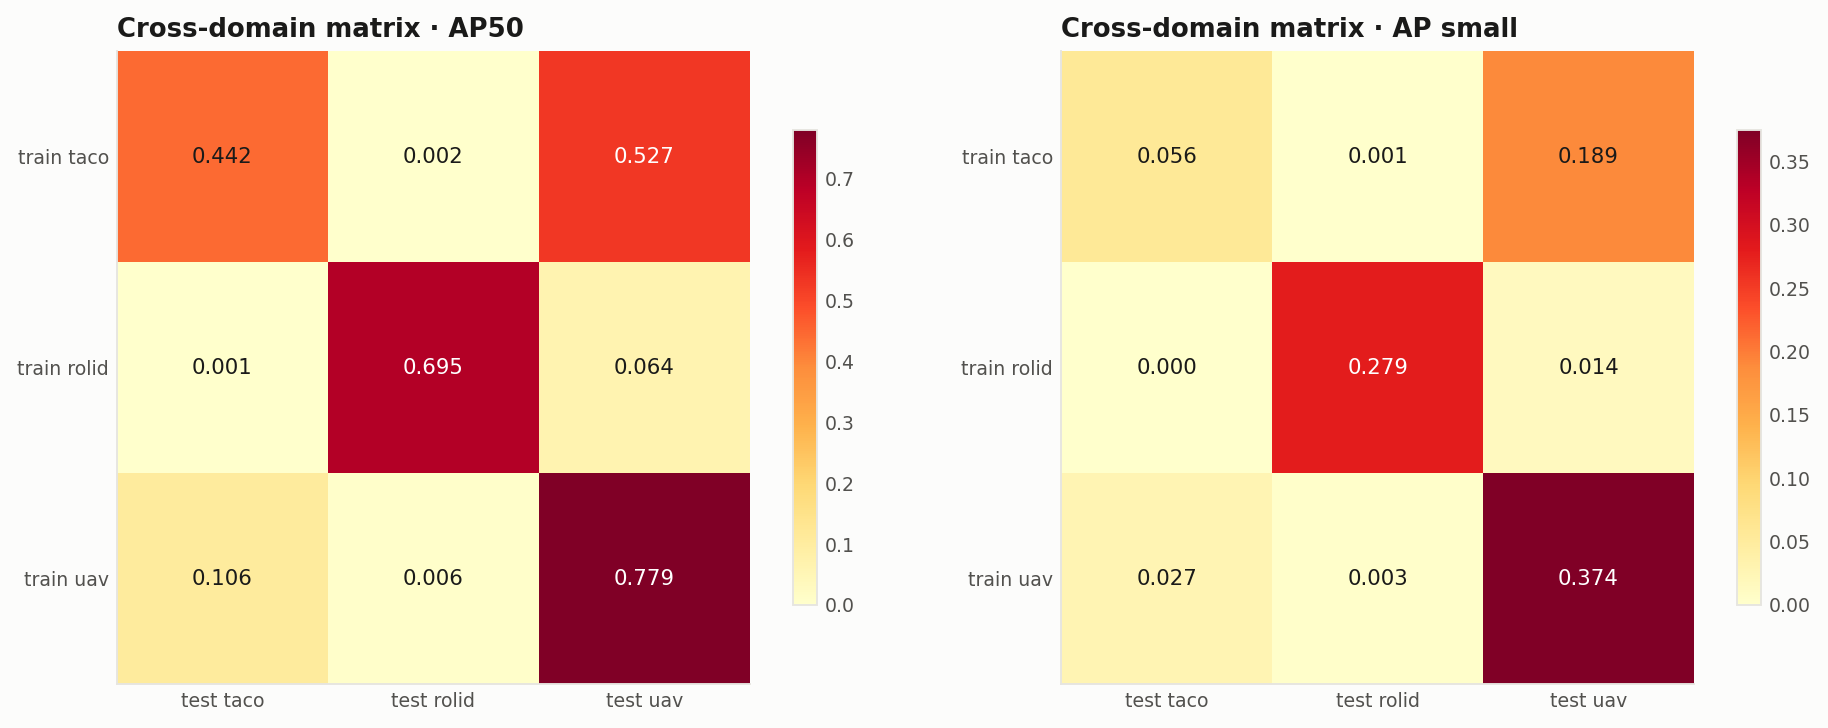
\includegraphics[width=0.80\linewidth]{matriz_cross_domain_final_en.png}
\end{center}
In-domain mean 0.639 AP$_{50}$; cross-domain 0.118. The dashcam domain is an
\textbf{island} (AP$_{50}\le 0.064$ both directions): its 22-px median object
falls below the smallest 32-px FPN anchor. Handheld$\rightarrow$drone retains
68\% scale, not appearance, dominates the gap.
}

\column{0.5}
\block{Split hygiene changes conclusions}{
\begin{center}
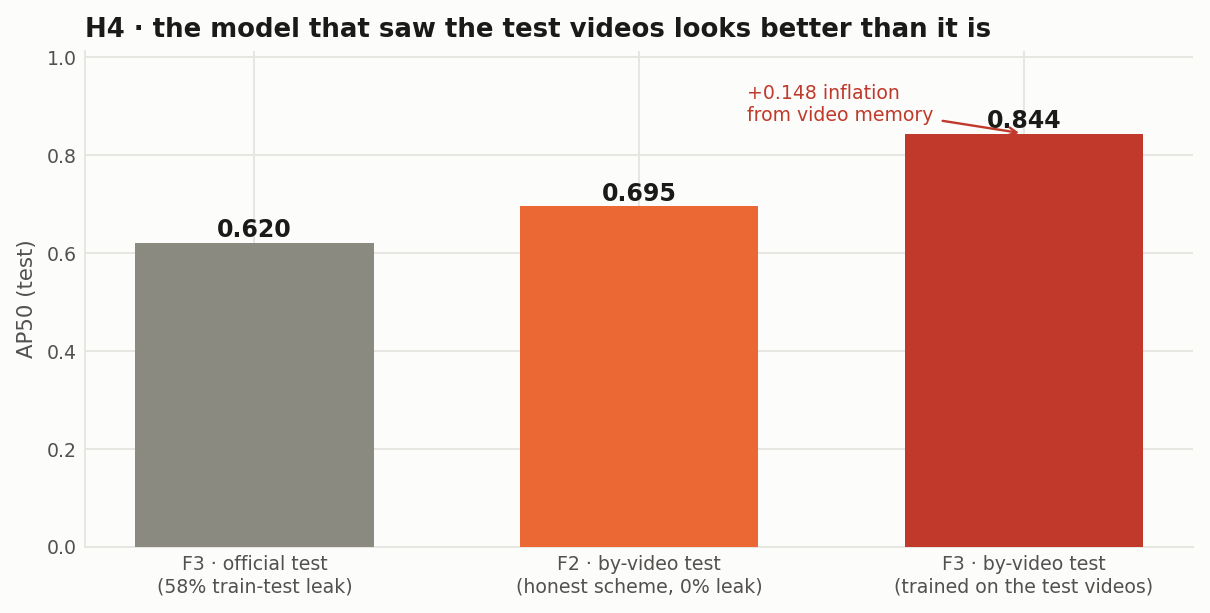
\includegraphics[width=0.58\linewidth]{fuga_oficial_vs_video_en.png}
\end{center}
On the \emph{same} clean test set, the model trained on the leaky official
split scores \textbf{0.844 vs.\ 0.695} for the cleanly trained one:
\textbf{+21\% relative} memorized scenes, not generalization. Group-aware
(by-video) splitting removes the bias at zero cost.
}
\end{columns}

% ═════════════════════ ROW 4 ═════════════════════
\begin{columns}
\column{0.5}
\block{Cheap levers: resolution}{
\begin{center}
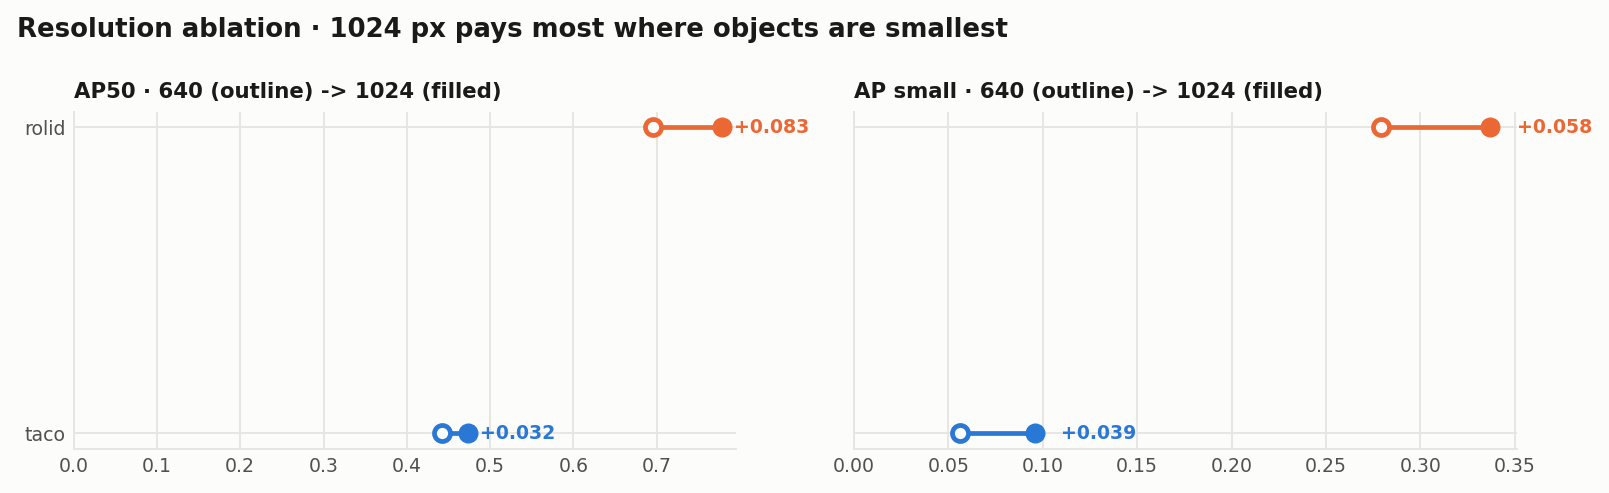
\includegraphics[width=0.85\linewidth]{ablacion_resolucion_en.png}
\end{center}
Gains concentrate where objects are smallest: dashcam +8.3 AP$_{50}$ /
+5.8 AP$_S$; handheld +3.2 / +3.9. Class granularity: excluding the marginal
glass class (38 test instances, AP$_{50}$ 0.049) lifts the remaining five
classes by +0.014 AP$_{50}$ on average.
}

\column{0.5}
\block{41M vs 2.6M parameters, same splits}{
\begin{center}
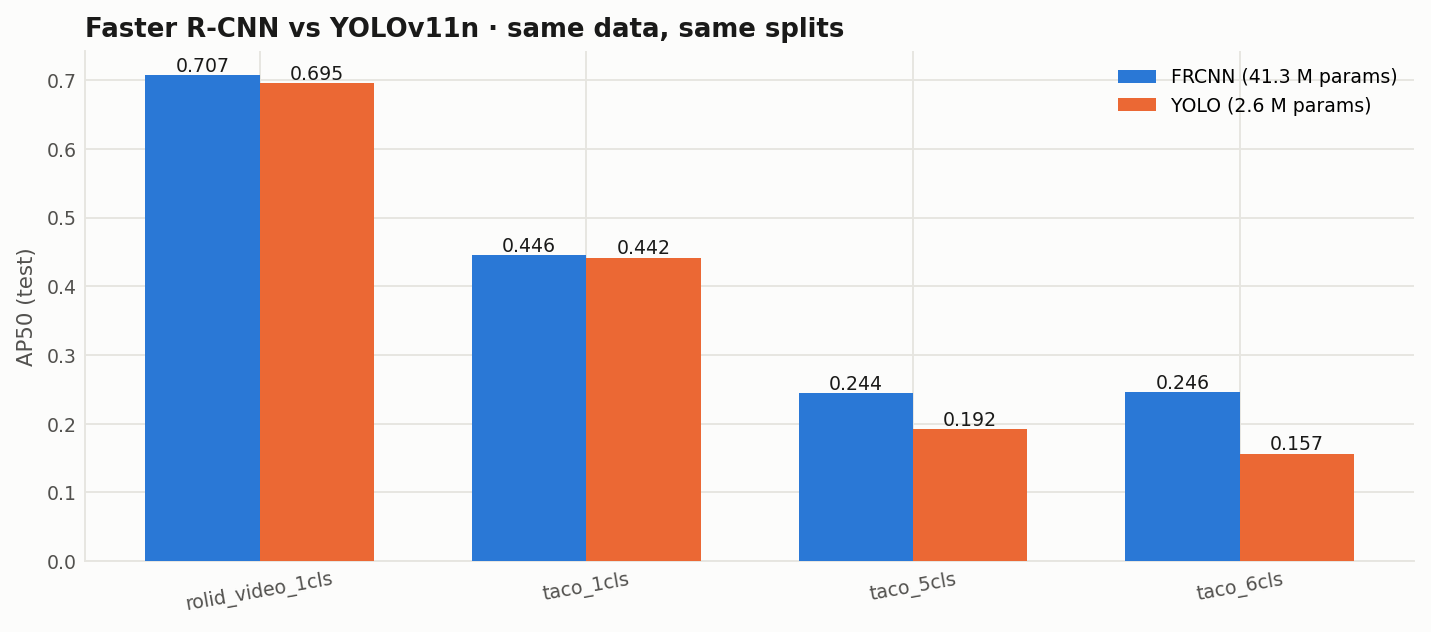
\includegraphics[width=0.70\linewidth]{comparativa_familias_en.png}
\end{center}
YOLOv11n stays within 1-4 AP$_{50}$ points of Faster R-CNN on single-class
litter (0.695 vs 0.707 dashcam) lightweight deployment is viable. The gap
widens on materials (0.157-0.192 vs 0.244-0.246). FCN: 0.577 test IoU;
VGG-16 crops: 97.8\% accuracy with CAM evidence on the object.
}
\end{columns}

% ═════════════════════ ROW 5 ═════════════════════
\begin{columns}
\column{0.58}
\block{Why they fail: TIDE error anatomy}{
\begin{center}
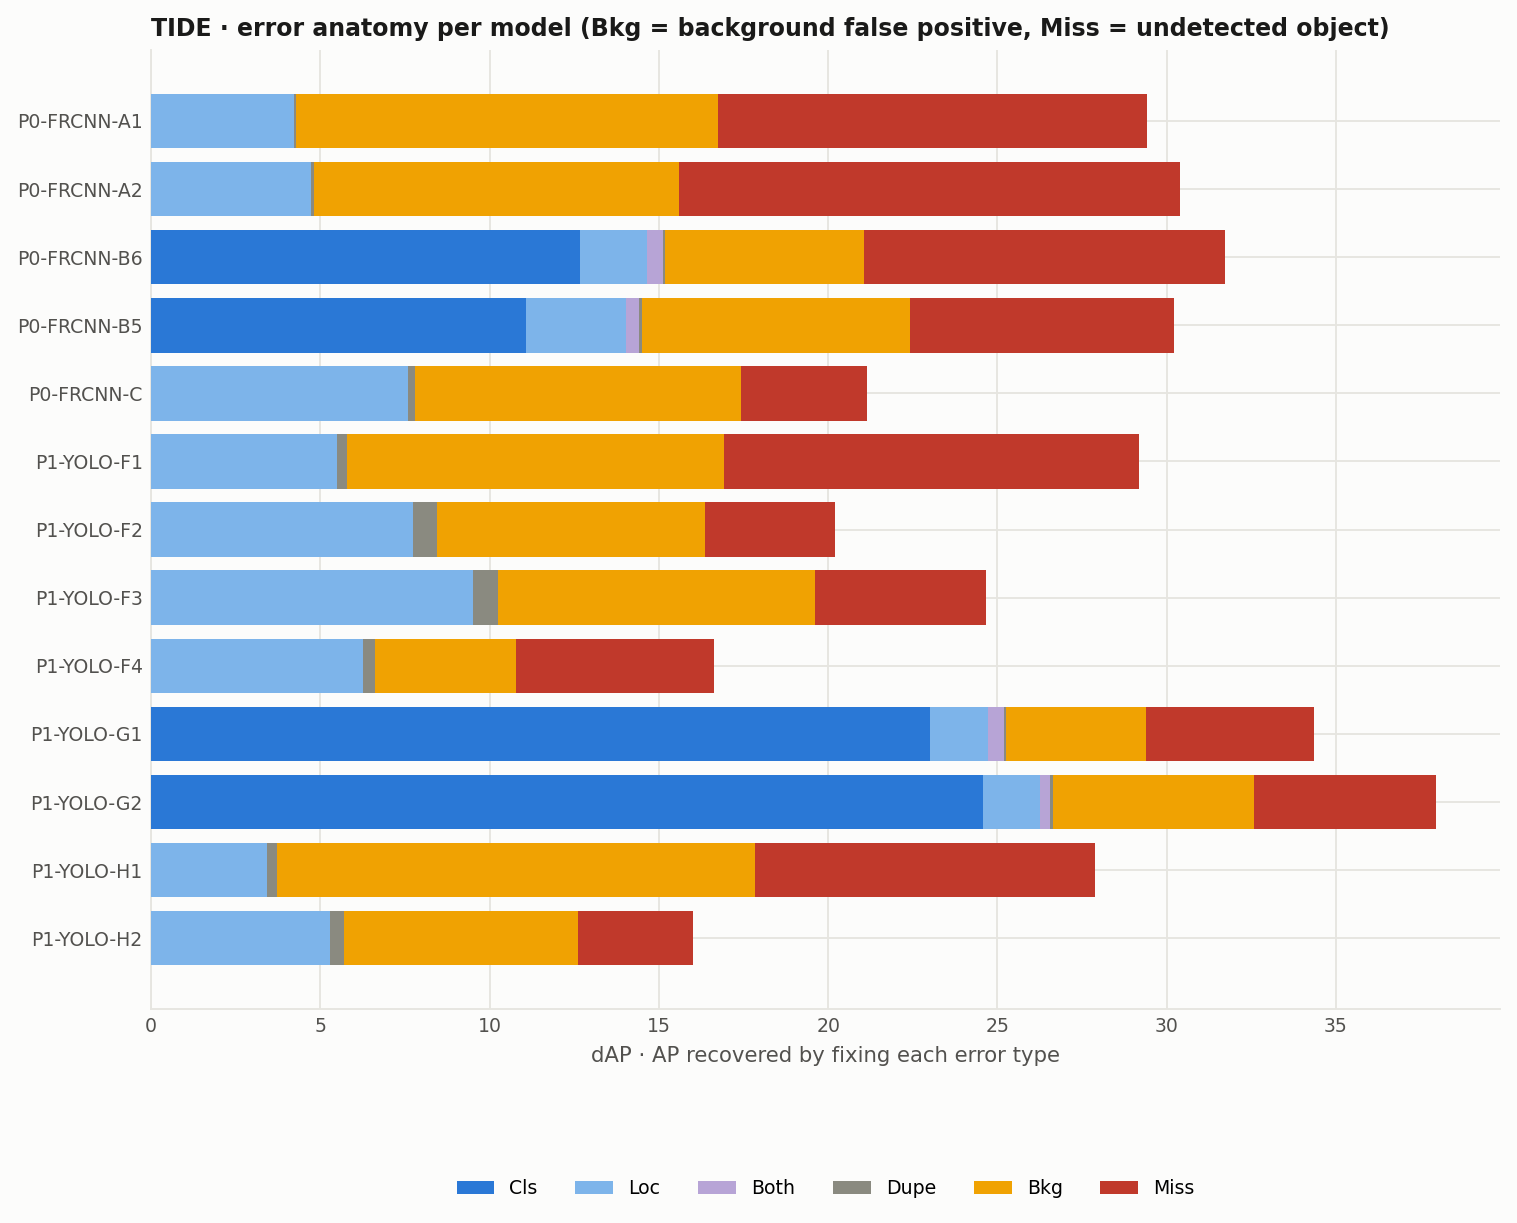
\includegraphics[width=0.42\linewidth]{tide_descomposicion_en.png}
\end{center}
Multiclass models lose up to \textbf{24.6 dAP to classification} vs.\ 1.7 to
localization naming the material, not finding the litter, is the
bottleneck; in-domain dashcam models miss little (dAP$_{\text{Miss}}\le 3.9$).
}

\column{0.42}
\block{Takeaways \& reproducibility}{
\begin{itemize}
\item \textbf{No universal litter model yet}: per-domain fine-tuning (or at
  least resolution adaptation) remains mandatory for mixed-sensor deployments.
\item \textbf{Audit before you train}: one hidden leak rewrites a benchmark;
  video/burst datasets should ship group identifiers.
\item \textbf{Detect class-agnostic, classify crops}: TIDE argues for
  decoupling material recognition (97.8\% on crops) from detection.
\end{itemize}
\vspace{3mm}
\textbf{Three released routes:} demo with pretrained weights on any photo
($\sim$5 min, CPU) \,·\, regenerate every paper number from artifacts
($\sim$10 min) \,·\, full pipeline from public data. Code, weights and
splits: \textbf{github.com released with the course hand-in.}
}
\end{columns}

\end{document}
